\documentclass[]{beamer}
%
% Choose how your presentation looks.
%
% For more themes, color themes and font themes, see:
% http://deic.uab.es/~iblanes/beamer_gallery/index_by_theme.html
%
\mode<presentation>
{
  \definecolor{StanfordCardinal}{RGB}{140, 21, 21} % Stanford Cardinal (primary)
  \usetheme{Madrid}      % or try Darmstadt, Madrid, Warsaw, ...
  \usecolortheme[named=StanfordCardinal]{structure} % or try albatross, beaver, crane, ...
  \usefonttheme{default}  % or try serif, structurebold, ...
  \setbeamertemplate{navigation symbols}{}
  \setbeamertemplate{caption}[numbered]
  %\useinnertheme{circles}
  %\useoutertheme{miniframes} % Alternatively: miniframes, infolines, split
} 
\usepackage{xcolor}
\usepackage[english]{babel}
\usepackage[utf8x]{inputenc}

\title[GSE Math Camp: Day 2]{GSE Math Camp Day 2: \\ Calculus}
\author{Klint Kanopka}
\institute{kkanopka@stanford.edu}
\date{Wednesday, September 4, 2019}

\begin{document}

    \begin{frame}
      \titlepage
    \end{frame}

    \begin{frame}{Math Camp Materials}
        All materials for the first week are hosted at:
        \url{http://github.com/klintkanopka/gsemathcamp}
    \end{frame}
    
    \begin{frame}{Outline}
      \tableofcontents
    \end{frame}

\section{Motivation}
    
    \begin{frame}{Motivation}
        Calculus is the study of (infinitesimal) change, and will be used in education research most often for optimization during model fitting. Understanding these concepts can help make courses like 400B, 430A, and 430B more clear. These ideas are also a prerequisite for the Econ 102 sequence, the Polisci 450 sequence, and any study of machine learning.
    \end{frame}

\section{Differentiation}
    \begin{frame}{Rates of Change}
        Our goal will be to find the rate of change of one quantity compared to another. \\
        \textbf{Key definitions/notations:} 
        \begin{itemize}
            \item<2-> Slope: the concept of slope as rate of change is important. For a straight line, the slope is \begin{center} {\LARGE $\frac{\text{rise}}{\text{run}} $} = {\LARGE $\frac{\text{change in y}}{\text{change in x}} $} = {\LARGE $\frac{\Delta{y}}{\Delta{x}}$ }\end{center}
            However, for other functions, the slope will not be constant.
        \item<3-> Derivative: can be thought of as the slope of a tangent line at a point on a function. The derivative tells you the rate of change at a point. It is denoted by {\LARGE $ \frac{\textit{dy}}{\textit{dx}}$} or f'(x) or y'. The value of the derivative may change for different values of x. In the graph below, we see that the derivative of function f(x) is positive, then 0, then negative (from left to right). 
    \end{itemize}
    \end{frame}

    \subsection{Intuition}

    \begin{frame}{Intuition}
        \begin{center} 
            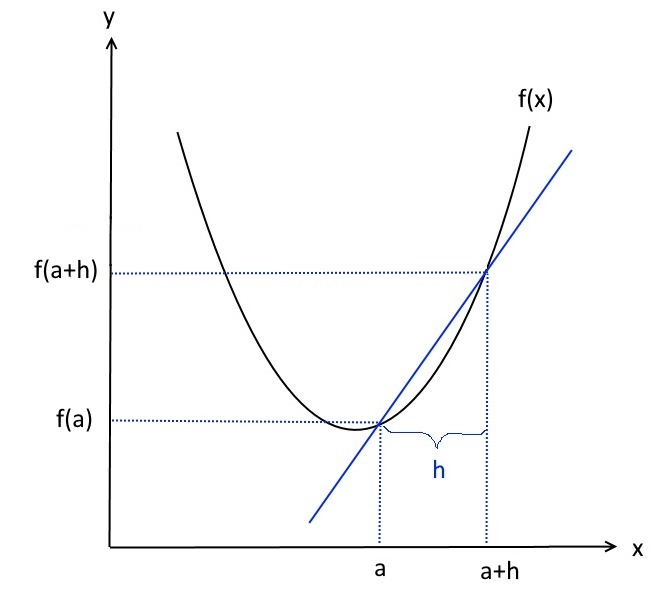
\includegraphics[scale=0.4]{img/calculus_diffquotient.jpg}
        \end{center}
    \end{frame}

    \begin{frame}{Formal Definition}
        For a function, $f(x)$, we define the derivative, $f'(x)$, as follows:
        $$f'(x) = \lim_{\Delta h\rightarrow 0}\frac{f(x+h)-f(x)}{h}$$
    \end{frame}

\subsection{Differentiation Rules}
    \begin{frame}{Common Differentiation Rules}
        \begin{enumerate}
            \item<2-> $(af)'=a(f')$
            \item<3-> $(f+g)'=f'+ g'$
            \item<4-> $(f-g)'=f'- g'$
            \item<5-> Product rule for $h(x)=f(x)g(x):  h'(x)=f'(x)g(x) + f(x)g'(x)$
            \item<6-> Chain rule for $h(x)=f(g(x)): h'(x)=f'(g(x))g'(x)$
            \item<7-> Exponents: If $f(x)=x^n$ then $f'(x)=nx^{n-1}$ and when n=0, f'(x)=0
            \item<8-> Log rules: $\frac{d}{dx} ln\;x = \frac{1}{x}$ and $\frac{d}{dx}e^{cx}=ce^{cx}$
        \end{enumerate}
    \end{frame}


    \begin{frame}{Practice}
        Find the derivative of each function with respect to $x$.
        \begin{enumerate}
            \item $f(x) = 7x^3 -3$
            \item $g(x) = 4x(5-x^2)$
            \item $h(x) = \frac{1}{x^4}$
            \item $f(x) = \ln x^2$
            \item $g(x) = \ln (x^2 + 1)$
            \item $h(x) = 6x^6 - 5x^5 + 4x^4 - 3x^3 + 2x^2 - x + 1$
        \end{enumerate}
    \end{frame}

\section{Integration}
\subsection{Motivating Example}
    \begin{frame}{Integrals}
    \begin{itemize}
        \item Our goal will be to find the area of a region $S$ that lies under the curve $f(x)$ from points $a$ to $b$.
        \item<2-> Suppose our function of interest is $f(x) = x^2 + 1$ on $x\in[0,2]$. Let's define the shaded region under $f(x)$ as $S$. \\
        \begin{center}
            \onslide<3->{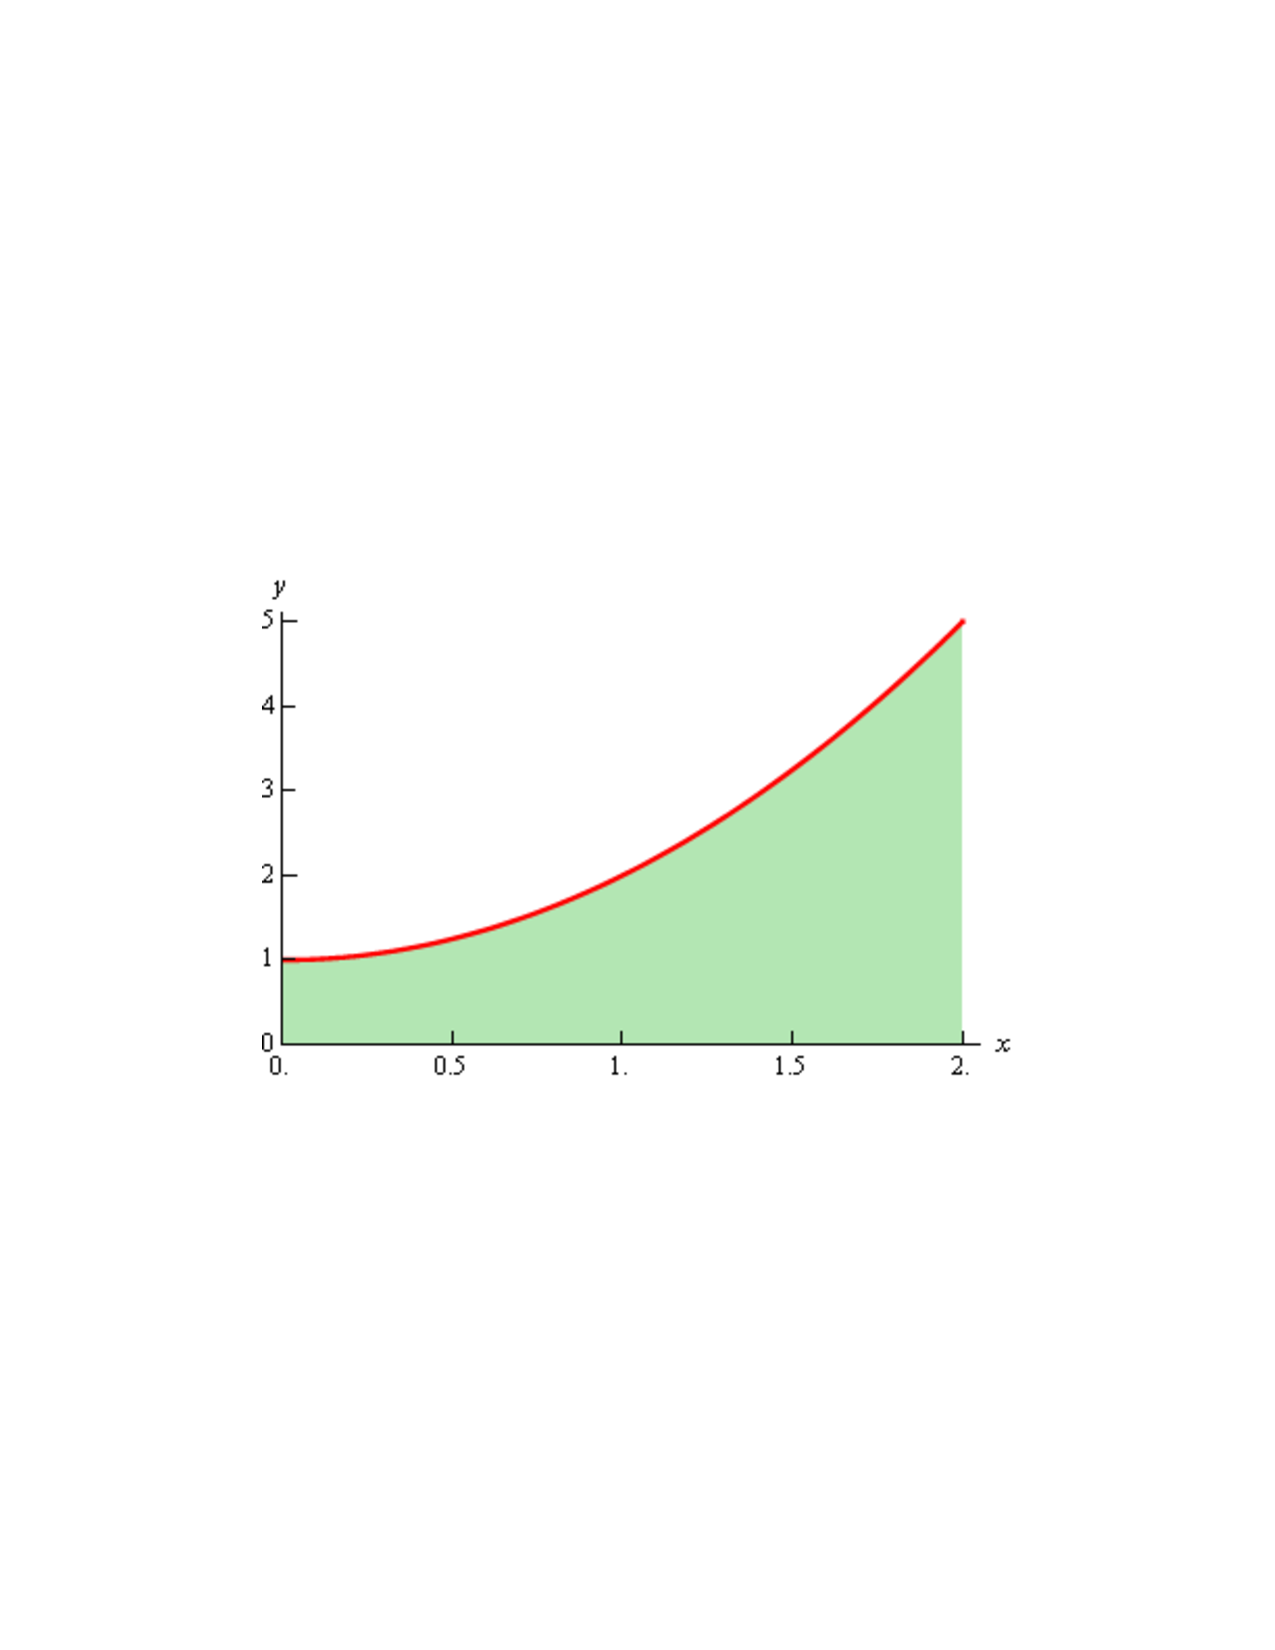
\includegraphics[scale=0.5]{img/integrals_mainfunction.pdf}}
        \end{center}
    \end{itemize}
    \end{frame}

    \begin{frame}{Estimating Areas}
    How can we find the area of $S$? We have a few options: \\
        \onslide<2->{Option 1: Rectangle method using right-hand endpoints: \\}
            \onslide<3->{\begin{center}
                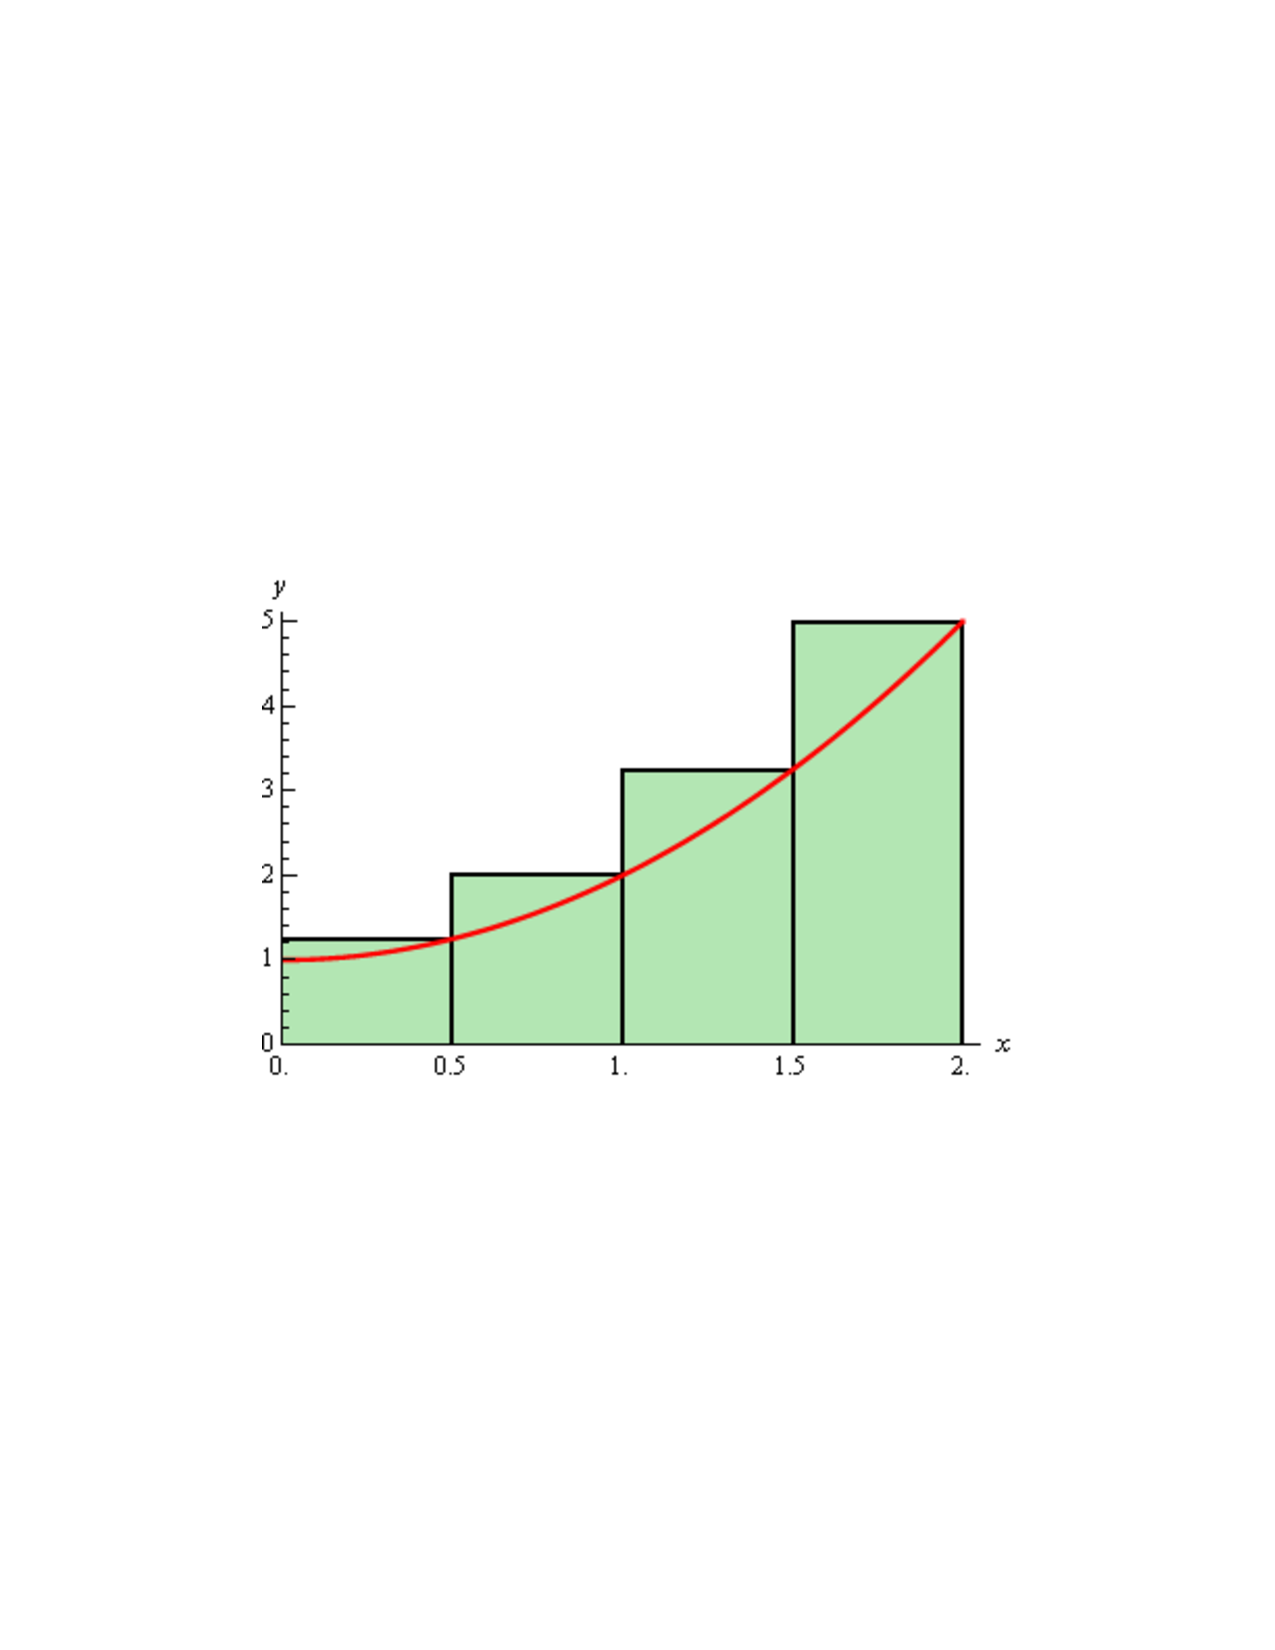
\includegraphics[scale=0.4]{img/integrals_rectangleR.pdf}
            \end{center}}
    \onslide<4->{\begin{align*}
    Area(S) &= \frac{1}{2}f\left(\frac{1}{2}\right) + \frac{1}{2}f\left(1\right) + \frac{1}{2}f\left(\frac{3}{2}\right) + \frac{1}{2}f\left(2\right) \\
    &= \frac{1}{2}\left(\frac{5}{4}\right) + \frac{1}{2}\left(2\right) + \frac{1}{2}\left(\frac{13}{4}\right) + \frac{1}{2}\left(5\right) \\
    &= 5.75
    \end{align*}}
    \end{frame}

    \begin{frame}{Estimating Areas}
    How can we find the area of $S$? We have a few options: \\
        \onslide<2->{Option 2: Rectangle method using left-hand endpoints: \\}
        \onslide<3->{\begin{center}
            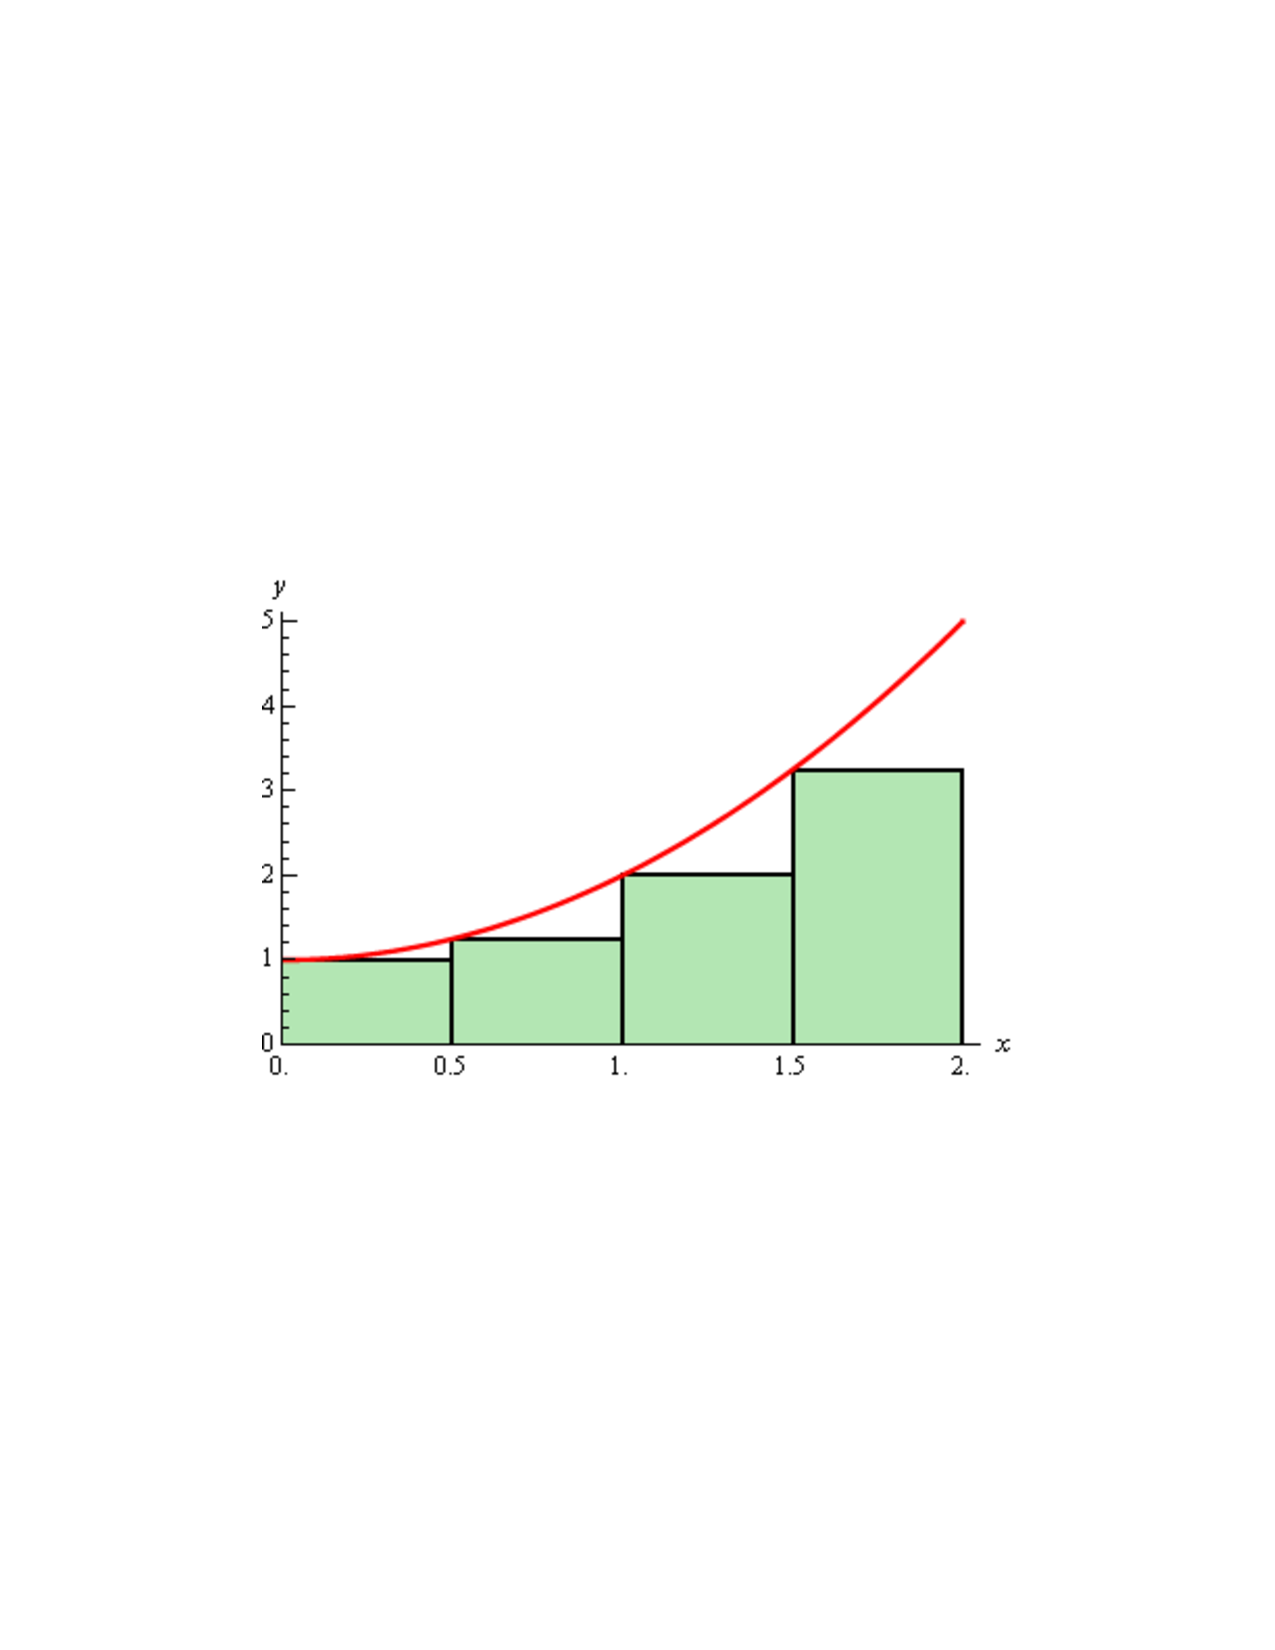
\includegraphics[scale=0.4]{img/integrals_rectangleL.pdf}\\
        \end{center}}
    \onslide<4->{Calculate $Area(S)$.}
    \end{frame}

    \begin{frame}{Estimating Areas}
        \onslide<2->{Rectangle method using midpoints: \\}
        \onslide<3->{\begin{center}
            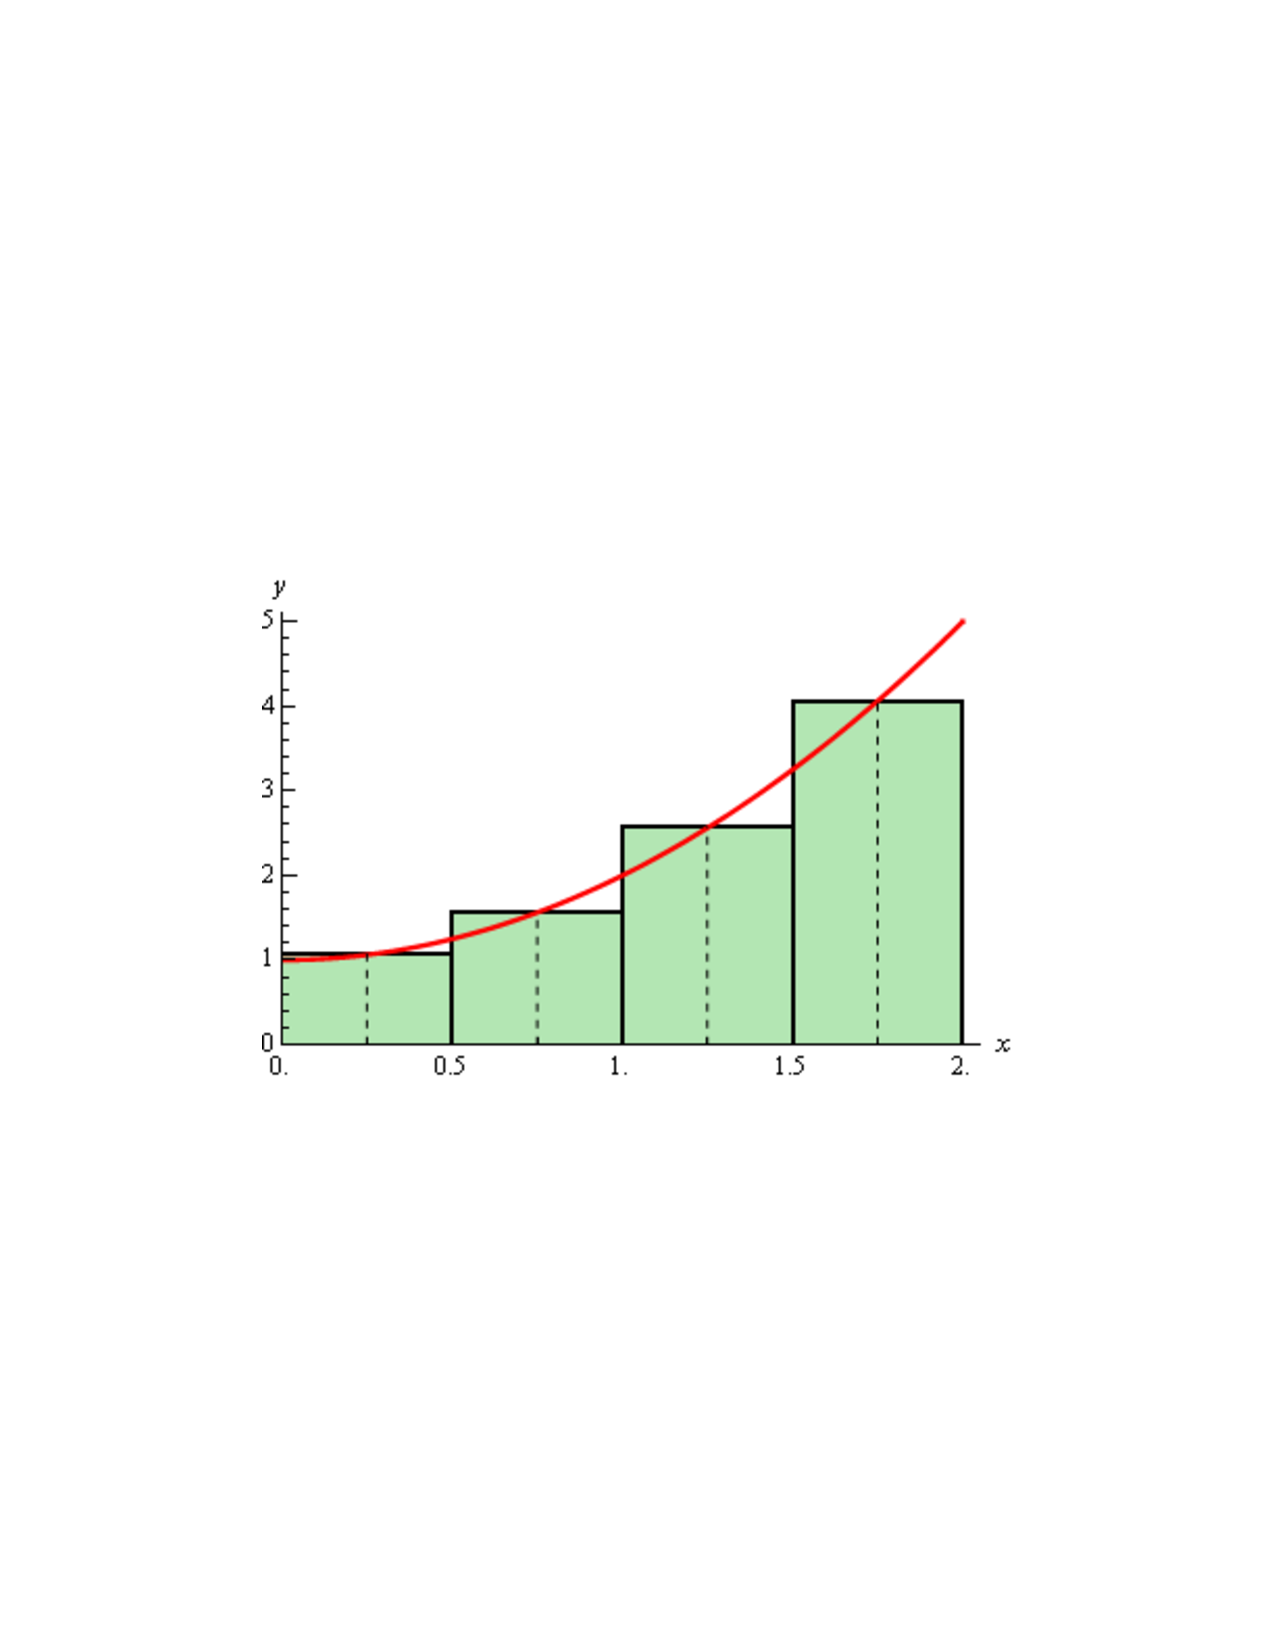
\includegraphics[scale=0.4]{img/integrals_midpoint.pdf}\\
        \end{center}}
        \onslide<4->{Calculate $Area(S)$.\\}
        \onslide<5->{Which other shapes might we try?}
    \end{frame}
    
    \begin{frame}{Doing Better}
        While we can use shapes like rectangles, our estimate of the area will be imprecise. One thing we might want to do is divide up our region into more parts. For example, using rectangles:

        \begin{center}
            \onslide<2->{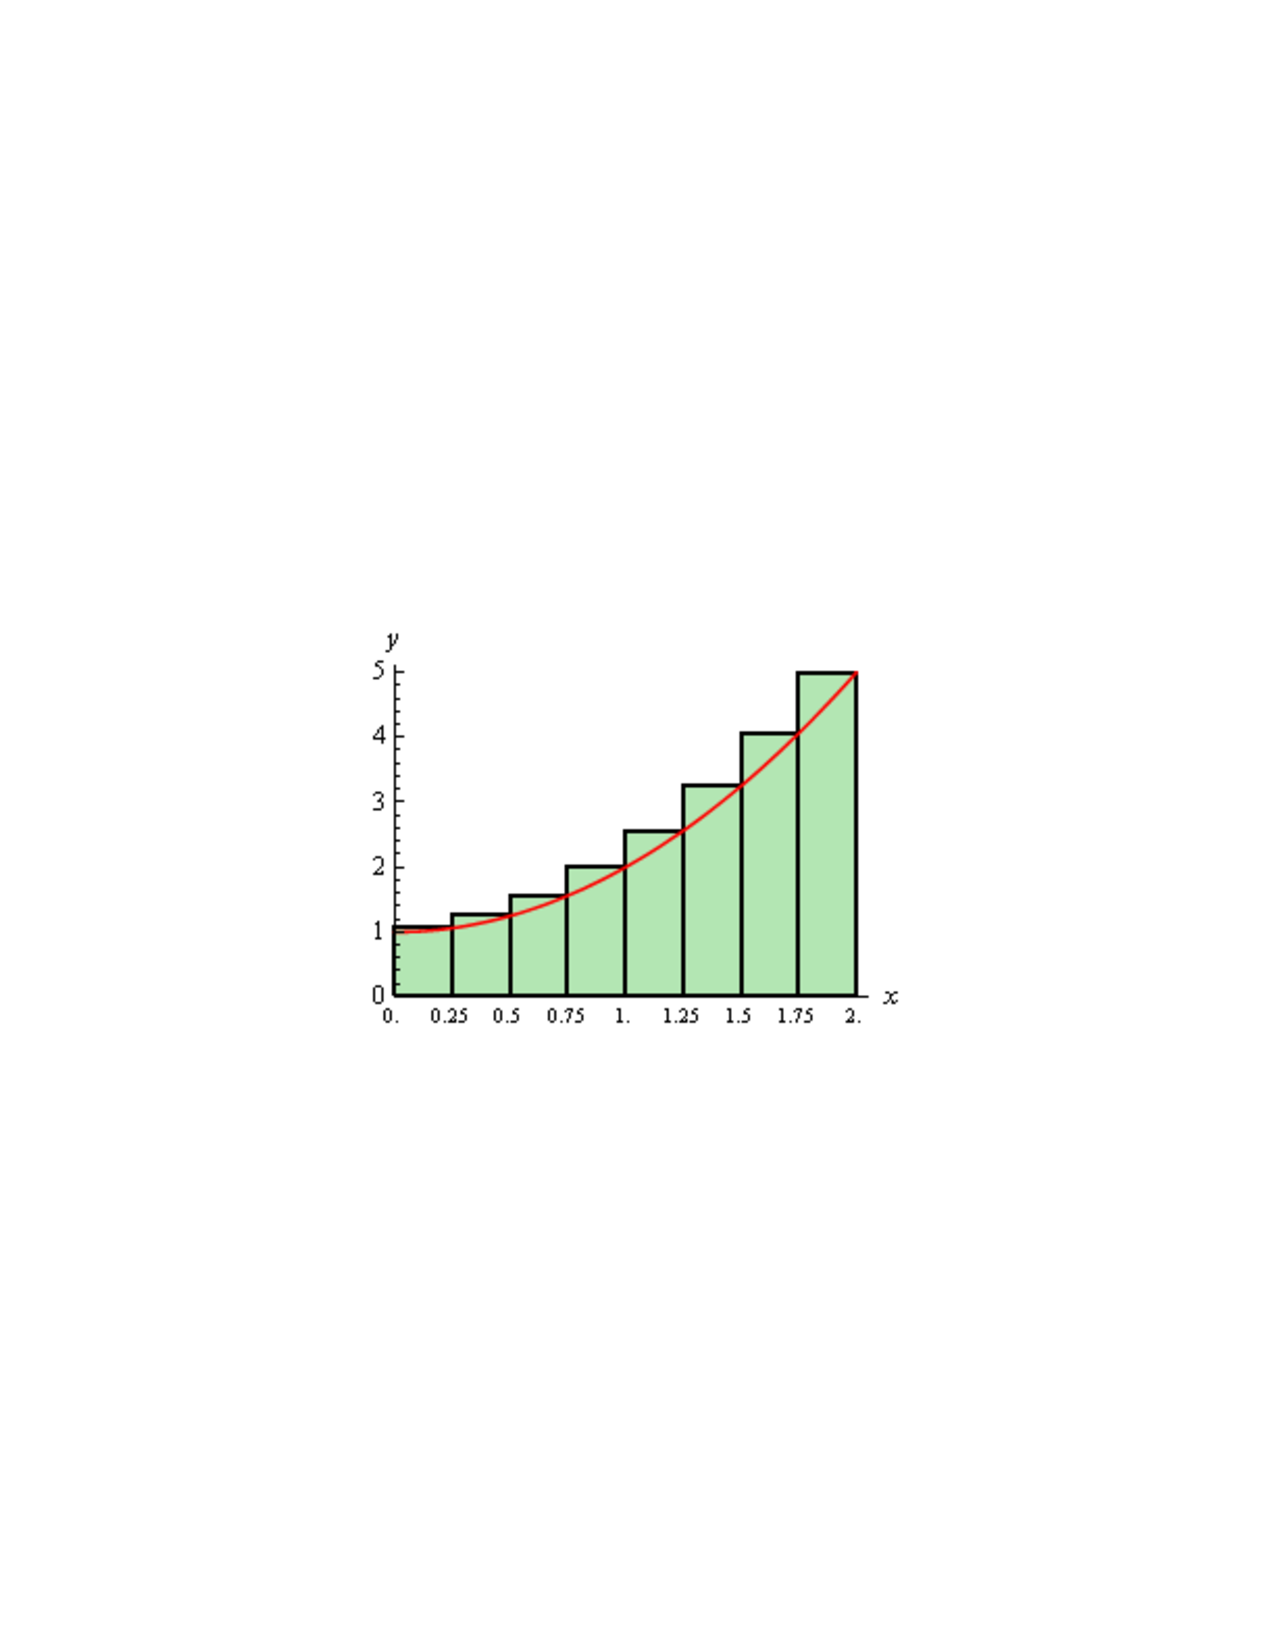
\includegraphics[scale=0.35]{img/integrals_morerectangleR.pdf}}
            \onslide<3->{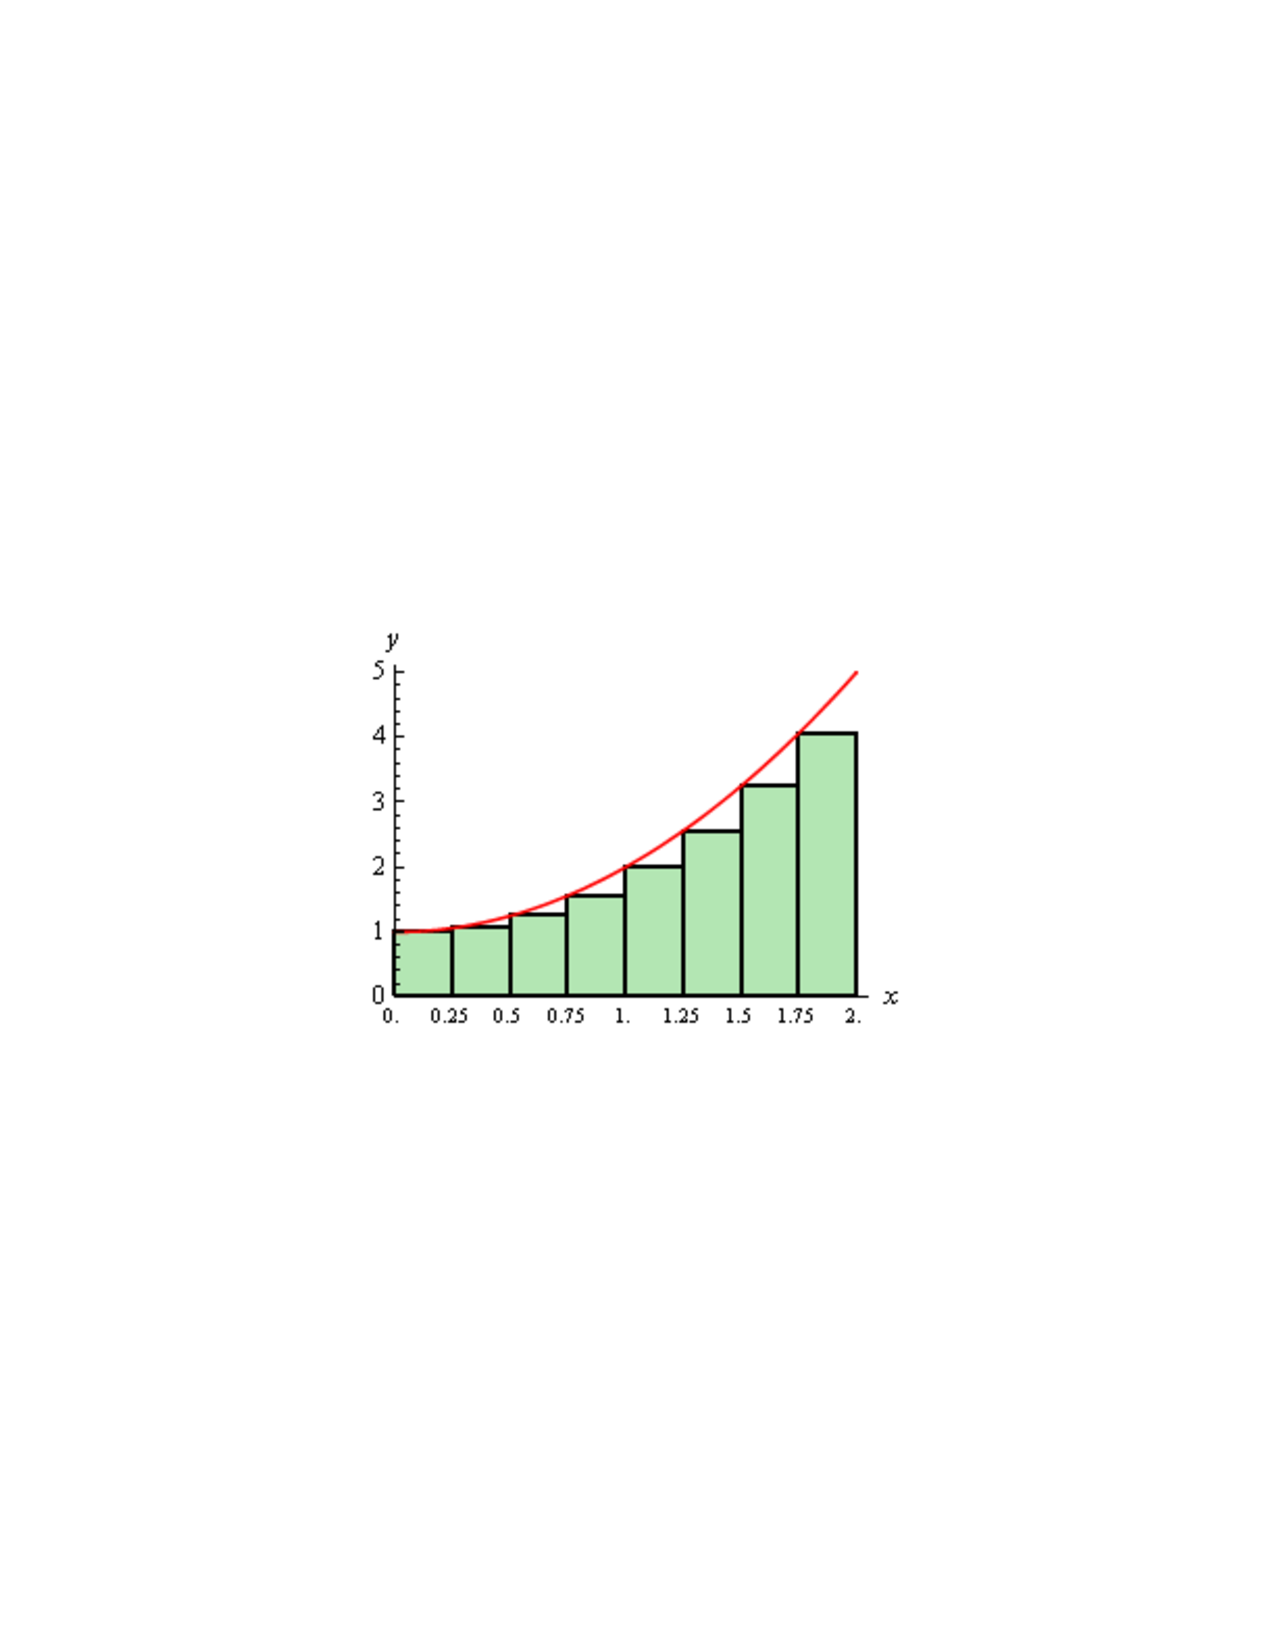
\includegraphics[scale=0.35]{img/integrals_morerectangleL.pdf}}
            \onslide<4->{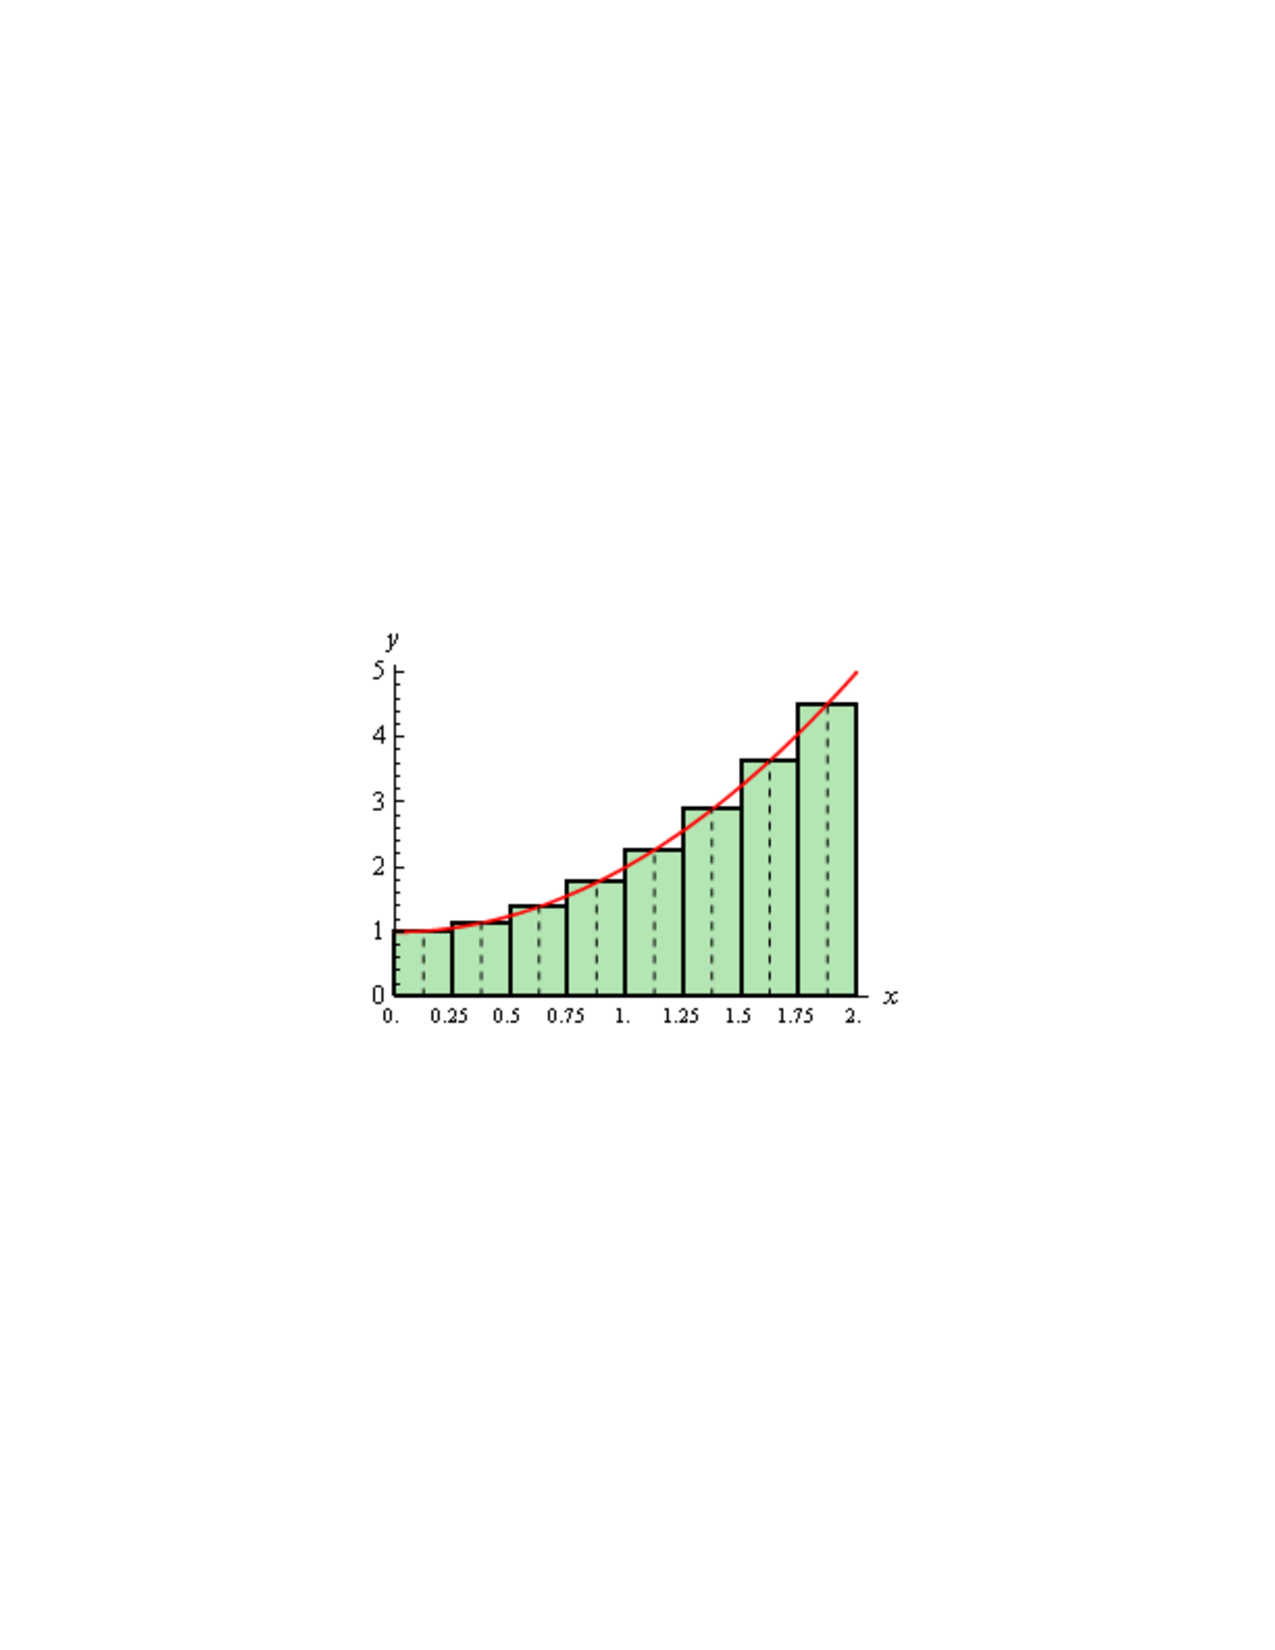
\includegraphics[scale=0.35]{img/integrals_moremidpoint.pdf}}
        \end{center}
        \onslide<5->{While dividing the region may get us closer to the true answer, it is still not exact!}
    \end{frame}

\subsection{Indefinite Integrals}


    \begin{frame}{Antiderivatives}
        Starting from a known function, $f$, we want to find a function $F$ for which $f$ is its derivative.
        \onslide<2->{Call $F$ the \textit{antiderivative} of $f$. We can write this as:}
            \onslide<3->{$$F' = f $$}
        \onslide<4->{\textbf{Definition}: If $F$ is the antiderivative of $f$, then $F$ is called the indefinite integral of $f$:}
            \onslide<5->{$$ F(x) = \int f(x) dx$$}
    \end{frame}

    \begin{frame}{Example}
        Let $f(x) = 6x$. We want to find $F(x) = \int 6x dx$.
        \onslide<2->{There are many potential solutions:}
        \begin{enumerate}
            \item<3-> $3x^2 + 1$
            \item<4-> $3x^2 + 2$
            \item<5-> $3x^2 + 100$, etc. 
        \end{enumerate}
        \onslide<6->{\textbf{IMPORTANT}: The derivative of a function can have many antiderivatives. With any antiderivative, we need to add a constant $c$, unless we are told that the antiderivative passes through a particular point. 

        The correct solution to our example problem, in the absence of any additional information, is $3x^2 + c$}
    \end{frame}

    \begin{frame}{Integration Rules}
        \begin{enumerate}
            \item<2-> $\int [(f(x) + g(x)] dx = \int f(x) dx + \int g(x) dx$
            \item<3-> $\int c f(x) dx = c \int f(x) dx$
            \item<4-> $\int x^n dx = \frac{x^{n+1}}{n+1} + c$
            \item<5-> $\int \frac{1}{x} dx = \ln|x| + c$ 
            \item<6-> $\int e^x dx = e^x + c$
            \item<7-> $\int e^{f(x)} f'(x) dx = e^{f(x)}+c$
            \item<8-> $\int [f(x)]^nf'(x) dx = \frac{1}{n+1}[f(x)]^{n+1}+c$
            \item<9-> $\int \frac{f'(x)}{f(x)} dx = \ln f(x) + c$
        \end{enumerate}
    \end{frame}
\subsection{Definite Integrals}
    \begin{frame}{Definite Integrals}
        We return to our initial problem of trying to calculate the area under a curve. Using an approximation method (i.e., one of the rectangle methods), we get close, but we want an exact answer.
        \begin{itemize}
            \item<2-> The rectangle approximation method is an application of a Riemann sum
                $$ Area(S) = \sum_{i=1}^n \underbrace{f(x_i)}_{height} \underbrace{\Delta x}_{base}$$
            \item<3-> How above making the base of the rectangles infinitesimally small? We can use limits:
                $$ Area(S) = \lim_{\Delta x\rightarrow 0} \sum_{i=1}^n \underbrace{f(x_i)}_{height} \underbrace{\Delta x}_{base}$$
        \end{itemize}
    \end{frame}

    \begin{frame}{Riemann Integral}
        The Riemann Integral is the solution to our problem!
            \onslide<2->{$$\int_a^b f(x) dx = \lim_{\Delta x\rightarrow 0} \sum_{i=1}^n f(x_i) \Delta x$$}
        \onslide<3->{The Riemann Integral is often referred to as the definite integral in calculus textbooks. Formally,  $\int_a^b f(x) dx$  denotes the integral of function $f$ from $a$ to $b$ (or the area under curve $f(x)$ from $x=a$ to $x=b$).}
    \end{frame}

    \begin{frame}{Fundamental Theorem of Calculus}
        Suppose $f$ is continuous on $[a,b]$,
            $$\int_a^b f(x) dx = F(b) - F(a)$$
        where $F$ is any antiderivative of $f$. That is, $F' = f$. 

        \onslide<2->{FTC II provides a way to calculate a definite integral:
        \begin{enumerate}
            \item Find the indefinite integral $F(x)$
            \item Evaluate $F(b) -F(a)$
        \end{enumerate}}
    \end{frame}
\subsection{Properties of Integrals}
    \begin{frame}{Properties of the Definite Integral}
        \begin{enumerate}
            \item<2-> $\int_a^a f(x) dx = 0 \quad \text{No area under a point.}$
            \item<3-> $\int_a^b f(x) dx = -\int_b^a f(x) \quad \text{Switching limits changes sign of the integral}$
            \item<4-> $\int_a^b [\alpha f(x) + \beta g(x)] dx = \alpha \int_a^b f(x) dx + \beta \int_a^b g(x) dx$
            \item<5-> $\int_a^b f(x) dx + \int_b^c f(x) dx = \int_a^c f(x) dx$
        \end{enumerate}
    \end{frame}

\end{document} 
